\chapter{Launch and manage instances}

Instances are virtual machines that run inside the cloud. You can launch
an \gls{instance} from the following sources:

\begin{itemize}
\item
  \begin{quote}
  Images uploaded to the Image service.
  \end{quote}
\item
  \begin{quote}
  Image that you have copied to a persistent volume. The instance
  launches from the volume, which is provided by the
  \textbf{cinder-volume} API through iSCSI.
  \end{quote}
\item
  \begin{quote}
  Instance snapshot that you took.
  \end{quote}
\end{itemize}

\strong{Launch an instance}\label{launch-an-instance}

\begin{enumerate}
\def\labelenumi{\arabic{enumi}.}
\item
  \begin{quote}
  Log in to the dashboard.
  \end{quote}
\item
  \begin{quote}
  Select the appropriate project from the drop down menu at the top
  left.
  \end{quote}
\item
  \begin{quote}
  On the Project tab, open the Compute tab and click Instances category.
  \end{quote}
\end{enumerate}

\begin{quote}
The dashboard shows the instances with its name, its private and
floating IP addresses, size, status, task, power state, and so on.
\end{quote}

\begin{enumerate}
\def\labelenumi{\arabic{enumi}.}
\item
  \begin{quote}
  Click Launch Instance.
  \end{quote}
\item
  \begin{quote}
  In the Launch Instance dialog box, specify the following values:
  \end{quote}
\end{enumerate}

\begin{center}
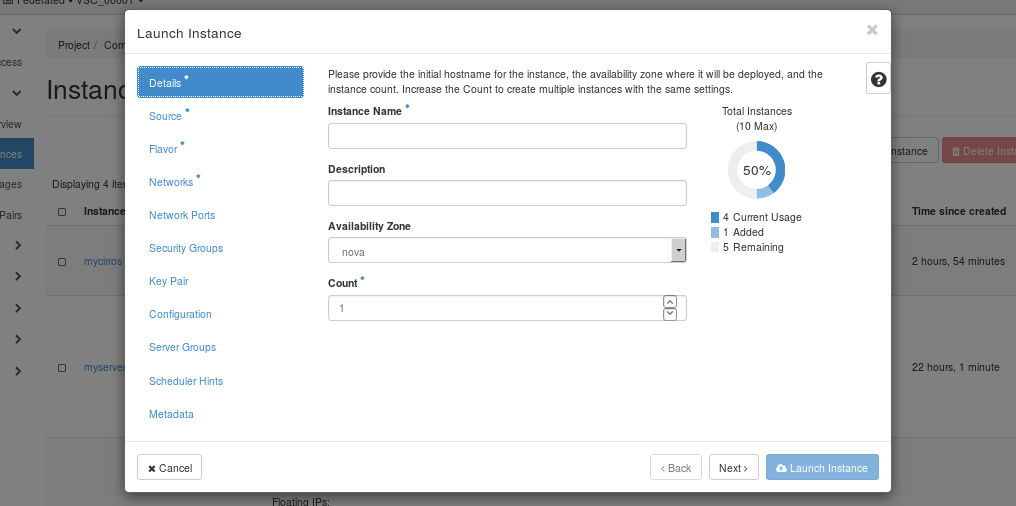
\includegraphics[scale=0.5]{img/tab-compute-instances-launch.png}
\end{center}


\begin{quote}
Details tab

\textbf{Instance Name}

Assign a name to the virtual machine.

~

Note

The name you assign here becomes the initial host name of the server. If
the name is longer than 63 characters, the Compute service truncates it
automatically to ensure dnsmasq works correctly.

After the server is built, if you change the server name in the API or
change the host name directly, the names are not updated in the
dashboard.

Server names are not guaranteed to be unique when created so you could
have two instances with the same host name.

\textbf{Description}

You can assign a brief description of the virtual machine.

\textbf{Availability Zone}

By default, this value is set to the availability zone given by the
cloud provider (for example, \textbf{us-west} or \textbf{apac-south}).
For some cases, it could be \textbf{nova}.

\textbf{Count}

To launch multiple instances, enter a value greater than \textbf{1}. The
default is \textbf{1}.

Source tab

\textbf{Instance Boot Source}

Your options are:

\textbf{Boot from image}

If you choose this option, a new field for Image Name displays. You can
select the image from the list.

\textbf{Boot from snapshot}

If you choose this option, a new field for Instance Snapshot displays.
You can select the snapshot from the list.

\textbf{Boot from volume}

If you choose this option, a new field for Volume displays. You can
select the volume from the list.

\textbf{Boot from image (creates a new volume)}

With this option, you can boot from an image and create a volume by
entering the Device Size and Device Name for your volume. Click the
Delete Volume on Instance Delete option to delete the volume on deleting
the instance.

\textbf{Boot from volume snapshot (creates a new volume)}

Using this option, you can boot from a volume snapshot and create a new
volume by choosing Volume Snapshot from a list and adding a Device Name
for your volume. Click the Delete Volume on Instance Delete option to
delete the volume on deleting the instance.

\textbf{Image Name}

This field changes based on your previous selection. If you have chosen
to launch an instance using an image, the Image Name field displays.
Select the image name from the dropdown list.

\textbf{Instance Snapshot}

This field changes based on your previous selection. If you have chosen
to launch an instance using a snapshot, the Instance Snapshot field
displays. Select the snapshot name from the dropdown list.

\textbf{Volume}

This field changes based on your previous selection. If you have chosen
to launch an instance using a volume, the Volume field displays. Select
the volume name from the dropdown list. If you want to delete the volume
on instance delete, check the Delete Volume on Instance Delete option.

Flavor tab

\textbf{Flavor}

Specify the size of the instance to launch.

~

Note

The flavor is selected based on the size of the image selected for
launching an instance. For example, while creating an image, if you have
entered the value in the Minimum RAM (MB) field as 2048, then on
selecting the image, the default flavor is \textbf{m1.small}.

Networks tab

\textbf{Selected Networks}

To add a network to the instance, click the + in the Available field.

Network Ports tab

\textbf{Ports}

Activate the ports that you want to assign to the instance.

Security Groups tab

\textbf{Security Groups}

Activate the security groups that you want to assign to the instance.

Security groups are a kind of cloud firewall that define which incoming
network traffic is forwarded to instances.

If you have not created any security groups, you can assign only the
default security group to the instance.

Key Pair tab

\textbf{Key Pair}

Specify a key pair.

If the image uses a static root password or a static key set (neither is
recommended), you do not need to provide a key pair to launch the
instance.

Configuration tab

\textbf{Customization Script Source}

Specify a customization script that runs after your instance launches.

Metadata tab

\textbf{Available Metadata}

Add Metadata items to your instance.
\end{quote}

\begin{enumerate}
\def\labelenumi{\arabic{enumi}.}
\item
  \begin{quote}
  Click Launch Instance.
  \end{quote}
\end{enumerate}

\begin{quote}
The instance starts on a compute node in the cloud.
\end{quote}

~

Note

If you did not provide a key pair, security groups, or rules, users can
access the instance only from inside the cloud through VNC. Even pinging
the instance is not possible without an ICMP rule configured.

You can also launch an instance from the Images or Volumes category when
you launch an instance from an image or a volume respectively.

When you launch an instance from an image, OpenStack creates a local
copy of the image on the compute node where the instance starts.

For details on creating images, see
\href{https://docs.openstack.org/image-guide/create-images-manually.html}{\emph{Creating
images manually}} in the \emph{OpenStack Virtual Machine Image Guide}.

When you launch an instance from a volume, note the following steps:

\begin{itemize}
\item
  \begin{quote}
  To select the volume from which to launch, launch an instance from an
  arbitrary image on the volume. The arbitrary image that you select
  does not boot. Instead, it is replaced by the image on the volume that
  you choose in the next steps.
  \end{quote}
\end{itemize}

\begin{quote}
To boot a Xen image from a volume, the image you launch in must be the
same type, fully virtualized or paravirtualized, as the one on the
volume.
\end{quote}

\begin{itemize}
\item
  \begin{quote}
  Select the volume or volume snapshot from which to boot. Enter a
  device name. Enter \textbf{vda} for KVM images or \textbf{xvda} for
  Xen images.
  \end{quote}
\end{itemize}

~

Note

When running QEMU without support for the hardware virtualization, set
\textbf{cpu\_mode="none"} alongside \textbf{virt\_type=qemu} in
\textbf{/etc/nova/nova-compute.conf} to solve the following error:

libvirtError: unsupported configuration: CPU mode 'host-model'

for ``x86\_64`` qemu domain on ``x86\_64`` host is not supported by
hypervisor

\strong{Connect to your instance by using SSH}\label{connect-to-your-instance-by-using-ssh}

To use SSH to connect to your instance, use the downloaded keypair file.

~

Note

The user name is \textbf{ubuntu} for the Ubuntu cloud images on
TryStack.

\begin{enumerate}
\def\labelenumi{\arabic{enumi}.}
\item
  \begin{quote}
  Copy the IP address for your instance.
  \end{quote}
\item
  \begin{quote}
  Use the \textbf{ssh} command to make a secure connection to the
  instance. For example:
  \end{quote}
\item
  \begin{quote}
  \$ ssh -i MyKey.pem ubuntu@10.0.0.2
  \end{quote}
\item
  \begin{quote}
  At the prompt, type \textbf{yes}.
  \end{quote}
\end{enumerate}

It is also possible to SSH into an instance without an SSH keypair, if
the administrator has enabled root password injection. For more
information about root password injection, see
\href{https://docs.openstack.org/nova/\osversion/admin/admin-password-injection.html}{\emph{Injecting the administrator password}} in the \emph{OpenStack Administrator
Guide}.

\strong{Track usage for instances}\label{track-usage-for-instances}

You can track usage for instances for each project. You can track costs
per month by showing meters like number of vCPUs, disks, RAM, and uptime
for all your instances.

\begin{enumerate}
\def\labelenumi{\arabic{enumi}.}
\item
  \begin{quote}
  Log in to the dashboard.
  \end{quote}
\item
  \begin{quote}
  Select the appropriate project from the drop down menu at the top
  left.
  \end{quote}
\item
  \begin{quote}
  On the Project tab, open the Compute tab and click Overview category.
  \end{quote}
\item
  \begin{quote}
  To query the instance usage for a month, select a month and click
  Submit.
  \end{quote}
\item
  \begin{quote}
  To download a summary, click Download CSV Summary.
  \end{quote}
\end{enumerate}

\strong{Create an instance snapshot}\label{create-an-instance-snapshot}

\begin{enumerate}
\def\labelenumi{\arabic{enumi}.}
\item
  \begin{quote}
  Log in to the dashboard.
  \end{quote}
\item
  \begin{quote}
  Select the appropriate project from the drop down menu at the top
  left.
  \end{quote}
\item
  \begin{quote}
  On the Project tab, open the Compute tab and click the Instances
  category.
  \end{quote}
\item
  \begin{quote}
  Select the instance from which to create a snapshot.
  \end{quote}
\item
  \begin{quote}
  In the actions column, click Create Snapshot.
  \end{quote}
\item
  \begin{quote}
  In the Create Snapshot dialog box, enter a name for the snapshot, and
  click Create Snapshot.
  \end{quote}
\end{enumerate}

\begin{quote}
The Images category shows the instance snapshot.
\end{quote}

To launch an instance from the snapshot, select the snapshot and click
Launch. Proceed with launching an instance.

\strong{Manage an instance}\label{manage-an-instance}

\begin{enumerate}
\def\labelenumi{\arabic{enumi}.}
\item
  \begin{quote}
  Log in to the dashboard.
  \end{quote}
\item
  \begin{quote}
  Select the appropriate project from the drop down menu at the top
  left.
  \end{quote}
\item
  \begin{quote}
  On the Project tab, open the Compute tab and click Instances category.
  \end{quote}
\item
  \begin{quote}
  Select an instance.
  \end{quote}
\item
  \begin{quote}
  In the menu list in the actions column, select the state.
  \end{quote}
\end{enumerate}

\begin{quote}
You can resize or rebuild an instance. You can also choose to view the
instance console log, edit instance or the security groups. Depending on
the current state of the instance, you can pause, resume, suspend, soft
or hard reboot, or terminate it.
\end{quote}
